\section{Data Life Cycle}

Throughout the literature, a variety of different definitions of data life cycle models can be found. Although they have been developed for different actuation domains, we describe here some of them which we think that can be applied for generic data, independently of its original domain.

\subsection{Data Documentation Initiative}

The first model to be analysed is the model proposed by Data Documentation Initiative (DDI). The DDI introduced a Combined Life Cycle Model for data managing \cite{data_documentation_initiative_overview_2008}. As Figure \ref{fig:ddi} shows, this model has eight elements or steps which can be summarized as follows, according to \cite{ball_review_2012}:

\begin{itemize}
    \item \textbf{Study concept.} At this stage, apart from choosing the research question and the methodology for collecting the data, the processing and analysis step of the needed data to answer the question is planned.
    \item \textbf{Data collection.} This model proposes different methods to collect data, like surveys, health records, statistics or Web-based collections.
    \item \textbf{Data processing.} At this stage, the collected data are processed to answer the proposed research question. The data may be recorded in both machine-readable and human-readable form.
    \item \textbf{Data archiving.} Both data and metadata should be archived to ensure long-term access to them, guaranteeing confidentiality.
    \item \textbf{Data distribution.} This stage involves the different ways in which data are distributed, as well as questions related to the terms of use of the used data or citation of the original sources. 
    \item \textbf{Data discovery.} Data may be published in different manners, through publications, web-indexes, etc.
    \item \textbf{Data analysis.} Data can be used by others to achieve different goals.
    \item \textbf{Repurposing.} Data can be used outside of their original framework, restructuring or combining it to satisfy diverse purposes.
\end{itemize}

%TODO: Vectorialize
\begin{figure}
    \center
    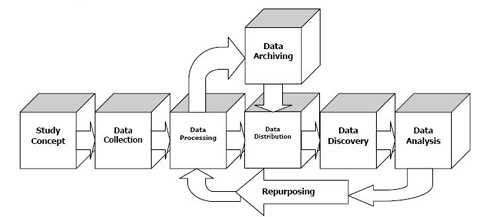
\includegraphics[width=\textwidth]{img/data_lifecycle/what-is-ddi-diagram.jpg}
    \caption{Combined Life Cycle Model (ownership: DDI Alliance).}
    \label{fig:ddi}
\end{figure}

%\footnotetext{\url{http://www.ddialliance.org/}}

\subsection{Australian National Data Service}

In late 2007, the \textit{Australian National Data Service} (ANDS) was founded with the objective of creating a national data management environment. ANDS established a set of verbs, denominated \textit{Data Sharing Verbs}, that describe the entire life cycle of the data \cite{burton_designing_2009}:

\begin{itemize}
    \item \textbf{Create.} \textit{Create} (or \textit{collect} for disciplines with an observational focus) is about the kinds of metadata that could be collected and the tools to fulfil this collection task.
    \item \textbf{Store.} This \textit{Data Sharing Verb} remarks the need for stable and web-accessible storage, taking care of the appropriate storing of data.
    \item \textbf{Describe.} The more information inside the storage, the more difficult its discovery, access and exploitation is. Annotating the data with the proper metadata solves this issue.
    \item \textbf{Identify.} The application of this verb implies the proper identification of each data resource, assigning a persistent identifier to each of them.
    \item \textbf{Register.} This step pertains to record the descriptions of the different data collections with one or more public catalogues.
    \item \textbf{Discover.} To improve data-reusing, ANDS suggests to enable different discovery services.
    \item \textbf{Access.} To guarantee the appropriate access to data, ANDS advises to provide a suitable search engine to retrieve these data. If data is not electronically available, ANDS recommends to provide contact details to get the data in conventional formats.
    \item \textbf{Exploit.} \textit{Exploit}, the final \textit{Data Sharing Verb}, comprises the tools, methodologies and support actions to enable reutilisation of data.
\end{itemize}

\subsection{Ecoinformatics data life cycle}

Michener and Jones define in \cite{michener_ecoinformatics:_2012} the concept of ``ecoinformatics'': \textit{a framework that enables scientists to generate new knowledge through innovative tools and approaches for discovering, managing, integrating, analysing, visualizing and preserving relevant biological, environmental, and socioeconomic data and information.} To manage these data, the following data life cycle has been defined, as can be seen at Figure \ref{fig:ecoinformatics}:
\begin{itemize}
    \item \textbf{Plan.} This step involves the confection of a data management planning.
    \item \textbf{Collect.} This step considers both manual (hand-written data sheets) and automatic (sensor networks) data-gathering methods.
    \item \textbf{Assure.} Quality assurance and quality control (QA/QC), an issue addressed in previously mentioned models is not taken into account. Michener and Jones proposal is based on developing methods to guarantee the integrity of  data. Quality assurance can also include the definition of standards for formats, codes, measurement units, metadata, etc.
    \item \textbf{Describe.} As other data life cycle models, this model remarks the value of the metadata to answer questions about \textit{who, when, where, how} and \textit{why}.
    \item \textbf{Preserve.} Data preservation implies the storage of the data and metadata, ensuring that these data can be verified, replicated and actively curated over time.
    \item \textbf{Discover.} The authors describe the data discovering process as \textit{one of the greatest challenges}, as many data are not immediately available because they are stored in individual laptops. The main challenges to publish the data in a proper way are related to the creation of catalogues and indexes, and about the implementation of the proper search engines.
    \item \textbf{Integrate.} Integrating data from different and heterogeneous sources can become a difficult task, as it requires \textit{understanding methodological differences, transforming data into a common representation, and manually converting and recording data to compatible semantics before analysis can begin}.
    \item \textbf{Analyze.} As well as the importance of a clear analysis step, this models remarks the importance of documenting this analysis with sufficient detail to enable its reproduction in different research frameworks.
\end{itemize}

\begin{figure}
    \center
    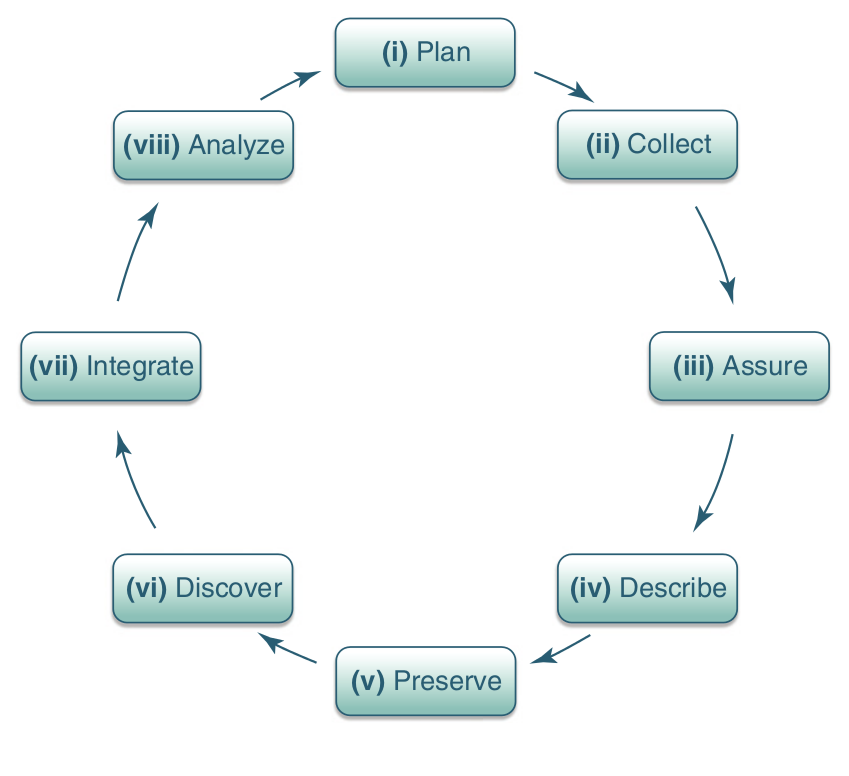
\includegraphics[scale=0.3]{img/data_lifecycle/ecoinformatics.png}
    \caption{Data life cycle in ecoinformatics. Taken from \cite{michener_ecoinformatics:_2012}.}
    \label{fig:ecoinformatics}
\end{figure}

\subsection{UK Data Archive}

Another data life cycle model is the one proposed by \textit{UK Data Archive}\footnote{\url{http://www.data-archive.ac.uk/create-manage/life-cycle}}. This model is oriented to help researchers publish their data in a manner that allows other researchers to continue their work independently. In Figure \ref{fig:uk-data-archive}, the following stages can be observed:
\begin{itemize}
    \item \textbf{Creating data.} Creating the data involves the design of the research question, planning how data are going to be managed and their sharing strategy. If we want to reuse existing data, we have to locate existing data and collect them. Whether data is new or existing, at this stage the metadata has to be created.
    \item \textbf{Processing data.} Like in other models, at this stage the data is translated, checked, validated and cleaned. In the case of confidential data, data needs to be ``anonymized''. The UK Data Archive recommends the creation of metadata at this stage too.
    \item \textbf{Analysing data.} At this stage data are interpreted and derived into visualizations or reports. In addition, the data are prepared for preservation, as mentioned in the following stage.
    \item \textbf{Preserving data.} To preserve data properly, they are migrated to the best format and stored in a suitable medium. In addition to the previously created metadata, the creating, processing, analysis and preserving processes are documented.
    \item \textbf{Giving access to data.} Once the data is stored, we have to distribute our data. Data distribution may involve controlling the access to them and establish a sharing license.
    \item \textbf{Re-using data.} At last, the data can be re-used enabling new research topics.
\end{itemize}

\begin{figure}
    \center
    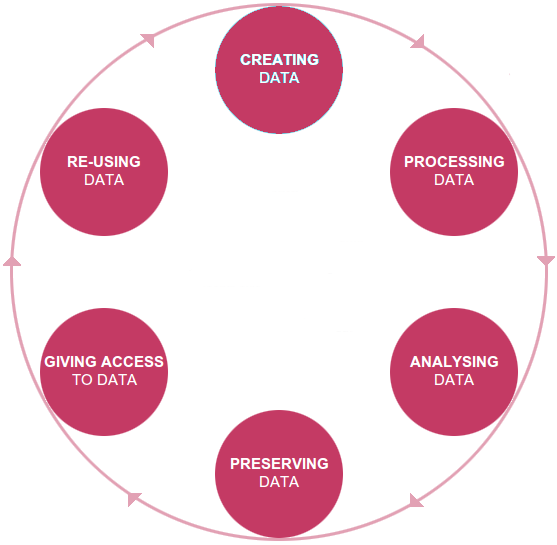
\includegraphics[scale=0.3]{img/data_lifecycle/uk-data-archive.png}
    \caption{Data life cycle proposed by UK Data Archive.}
    \label{fig:uk-data-archive}
\end{figure}

\subsection{The LOD2 Stack Data Life Cycle}

The last analyzed data life cycle has been developed under the LOD2\footnote{\url{http://lod2.eu/}} project. This project proposes a technological and methodological stack which supports the entire life cycle of Linked Data \cite{auer_managing_2012}. As Figure \ref{fig:lod2} shows, the proposed life cycle phases are the following:

\begin{figure}
    \center
    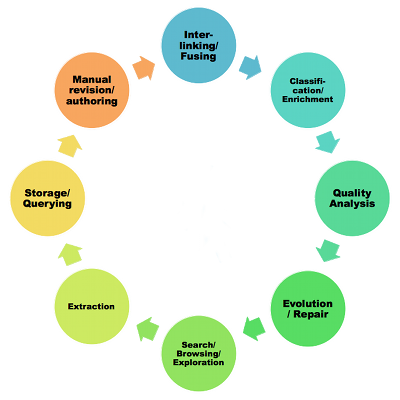
\includegraphics[scale=0.6]{img/data_lifecycle/lod2lifecyle1.png}
    \caption{Linked Data life cycle from LOD2 stack.}
    \label{fig:lod2}
\end{figure}

\begin{itemize}
    \item \textbf{Storage.} As RDF data presents more challenges than relational data, they propose the collaboration between known and new technologies, like columnstore technology, dynamic query optimization, adaptive caching of joins, optimized graph processing and cluster/cloud scalability.

    \item \textbf{Authoring.} LOD2 provides provenance about data collected through distributed social, semantic collaboration and networking techniques.

    \item \textbf{Interlinking.} At this phase, LOD2 offers approaches to manage the links between different data sources.

    \item \textbf{Classification.} This stage deals with the transformation of raw data into Linked Data. This transformation implies the linkage and integration of data with upper level ontologies.

    \item \textbf{Quality.} Like other models, LOD2 develops techniques for assesing quality based on different metrics.

    \item \textbf{Evolution/Repair.} At this stage, LOD2 deals with the dynamism of the data from the Web, managing changes and modifications over the data.

    \item \textbf{Search/Browsing/Exploration.} This stage is focused on offering Linked Data to final users through different search, browsing, exploration and visualization techniques.
\end{itemize}

\subsection{A common data life cycle for smart cities}

Based on these data life cycle models, we propose a common data life cycle for managing data in smart cities. As can be seen at Figure \ref{fig:model}, the different stages of mentioned models have been aggregated, forming our proposed model.
%\begin{table}
%    \centering
%    \begin{tabular}{|l|l|l|l|l|}
%        \hline
%        \textbf{DDI} & \textbf{ANDS} & \textbf{Ecoinformatics} & \textbf{UK Data Archive} & \\
%        \hline \hline
%        \rowcolor [gray]{.9} Study  concept & Create & Plan & Create & \\
%        \cellcolor [gray]{.9} Collect & \cellcolor [gray]{.8} Store & \cellcolor [gray]{.9} Collect & Process & \\
%        Process & Describe & Assure & Analyze & \\
%        Archive & Identify & Describe & Preserve & \\
%        Distribute & Register & Preserve & Access & \\
%        Discovery & Discover & Discover & Re-use & \\
%        Analysis & Access & Integrate & &  \\
%        Repurposing & Exploit & Analyze & & \\
%        \hline
%   \end{tabular}
%\end{table}

\begin{figure}
    \center
    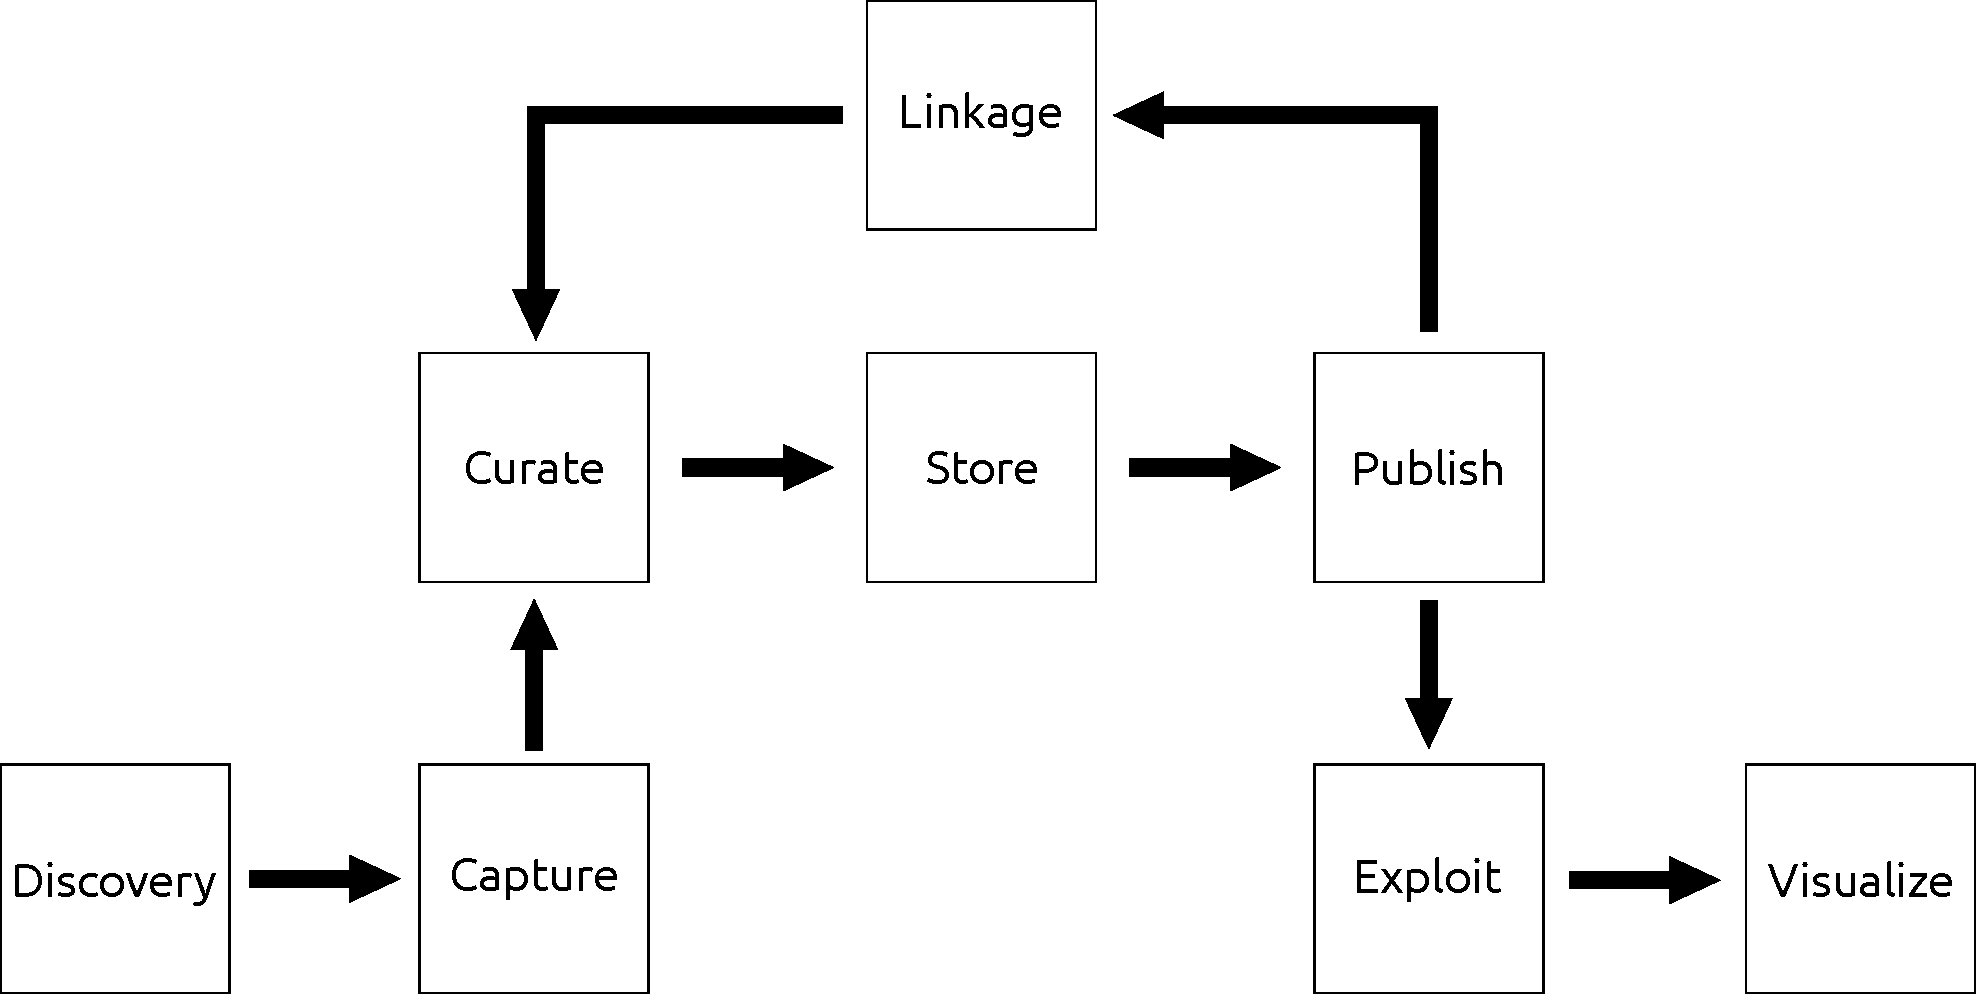
\includegraphics[width=0.60\linewidth]{img/data_lifecycle/model.pdf}
    \caption{Proposed model.}
    \label{fig:model}
\end{figure}

The different stages of this model, which are going to be explained widely in following sections, are:
\begin{itemize}
	\item \textbf{Discovery:} The first step in our model consists of discovering where data can be taken from, identifying the available datasets which contain the necessary data to accomplish our task. Datasources can either be maintained by us, or by external entities, so the more metadata we can gather from datasets, the easier further steps will become.
    \item \textbf{Capture:} Once datasources are identified, data needs to be collected. In a smart city environment, there are a lot of alternatives to capture data, like sensors, data published by public administration, social networks or in more traditional way like surveys.
    \item \textbf{Process:} After the required data are captured, they are prepared to be stored and in need of proper methods to explore them. This processing involves the analyzing, refining, cleaning, formatting and transformation of the data.
    \item \textbf{Store:} The storage of data is, probably, the most delicate action in the life cycle. Above the storage  all the analysis tools are build, and is the ``final endpoint'' when someone requests our data. A suitable storage should have indexing, replication, distribution and backup features, among other services.
    \item \textbf{Publish:} Most of the previously mentioned models prioritize the analysing stage over the publication stage. In our model, we defend the opposite approach for a very simple reason: when you consume your data before their publication, and using different processes as the rest of the people who is going to consume them, you are not making enough emphasis on publishing these data correctly. Everybody has ever met a research paper or an application in which accessing the data was difficult, or, when once the data was collected it became totally incomprehensible. To avoid this issue, we propose to publish the data before their consumption, following the same process the rest of the people does.
    \item \textbf{Linkage:} Before consuming data, we suggest to search for links and relationships with other datasets found in the discovery step. Actual solutions do not allow the linkage with unknown datasets, but tools are developed to ease link discovery processes between two or more given datasources.
    \item \textbf{Consume:} Once the data is published, we use the provided methods to consume the data. This data consumption involves data mining, analytics or reasoning.
    \item \textbf{Visualize:} To understand data properly, designing suitable visualizations is essential to show correlations between data and the conclusions of the data analysis in a human-understandable way.
    
\end{itemize}

